\CatchFileDef{\deltatable}{delta-table.tex}{}
\CatchFileDef{\deltatablesample}{delta-table-2.tex}{}
\CatchFileDef{\singlelenamsb}{single-res-table-msb-Lena.tex}{}
\CatchFileDef{\singlelenashr}{single-res-table-shr-Lena.tex}{}
\CatchFileDef{\singlelenadif}{single-res-table-dif-Lena.tex}{}


\section{Experimental results}

The experimental results for some commonly used test images are shown in Table~\ref{tab:common}. 
Within each column, there are three sub-columns representing the data of our method, the method of~\cite{Yin2020} and the difference, respectively.


explain -Yin...



In the column \emph{Ref}, our improvement of Section~\ref{sec:improveref} introduced almost a thousand bytes that can be used for information hiding for an $512 \times 512$ image, which turns into a contribution of averagely more than five thousand bits in \emph{Capacity}. 
%This improvement increases dramatically with cover images of larger size.

%In the column \emph{Label Map}, our improvement described in Section~\ref{sec:improvetree} created averagely more than five thousand bits for any $512 \times 512$ image.

explain why some plus

In the column \emph{Label Map}, our improvement described in Section~\ref{sec:improvetree} surely reduces the overall length of label map $T$. 
The detail of the special case of \emph{Man} $1024 \times 1024$ is demonstrated in Table~\ref{tab:man}.
It is understandable that $T$ is of size $1023 \times 1023$ when applying the method of Yin et al., 
while it is of size $1024 \times 1024 - (7 + 63)$ when applying our method. 
Since our method produces a larger $T$, it is inevitable that there will be a longer $T'$ for some images, as we have seem in column \emph{Label Map}. 
But if we further exam the coding result of \emph{Man} $1024 \times 1024$ in Table~\ref{tab:man}, our method still produce a slightly shorter average code length per value in $T$, which reflects the truth that our method produces a better Huffman coding tree.

Though we have to spend more space in $S^{header}$ to store the Huffman tree topology, we also remove the $LEN$ column, as discussed in Section~\ref{sec:improvesize}, hence $S^{header}$ remains almost the same size, as shown in the column \emph{Hdr}.



\begin{table}
	\scriptsize
	\centering
	\caption{Experimental results of sample images (Ours/Yin et~al./$\Delta$)}
	\label{tab:common}
	\begin{tabular}{l@{}c r@{/}r@{/}r r@{/}r@{/}r r@{/}r@{/}r r@{/}r@{/}r }
		\toprule
		\multicolumn{1}{c}{Image} & Size & 
		\multicolumn{3}{c}{Hdr(bit)}            & \multicolumn{3}{c}{Ref(byte)}& \multicolumn{3}{c}{Capacity(bit)}& \multicolumn{3}{c}{Label Map(bit)}      \\ 
		\midrule
		% paste from here ---------------------------------------------------------------
		
%		\deltatable
		
%		\midrule
		
		\deltatablesample
		
		% paste till here -----------------------------------------------------------------
		
		
		\bottomrule
	\end{tabular}
\end{table}

%\begin{table}
%	\tiny
%	\centering
%	\caption{Experimental results of test images (Ours/Yin et~al./$\Delta$)}
%	\label{tab:big6}
%	\begin{tabular}{@{}c@{\;}c@{\;}c@{/}c@{/}c r@{/}r@{/}r r@{/}r@{/}r r@{/}r@{/}r r@{/}r@{/}r}
%		\toprule
%		Image & Size & 
%		\multicolumn{3}{c}{Hdr(bit)}            & \multicolumn{3}{c}{Ref(byte)}& \multicolumn{3}{c}{Capacity(bit)}& \multicolumn{3}{c}{Label Map(bit)} & \multicolumn{3}{c}{BPP.}      \\ 
%		\midrule
%		% paste from here ---------------------------------------------------------------
%
%		\deltatable
%		
%		% paste till here -----------------------------------------------------------------
%		
%		
%		\bottomrule
%	\end{tabular}
%\end{table}






\begin{table}
%	\scriptsize
	\centering
	\caption{Experimental results of image datasets (Ours/Yin et~al./$\Delta$)}
	\label{tab:bestworst}
	\label{tab:exp3}
	\begin{tabular}{l c@{/}c@{/}c c@{/}c@{/}c c@{/}c@{/}c}
		\toprule
		BBP & \multicolumn{3}{c}{Best Case} & \multicolumn{3}{c}{Worst Case} & \multicolumn{3}{c}{Average} \\
		\midrule
		BOSSBase  &  6.881 &	5.898	&$+0.984$& 0.716&	0.665&	$+0.051$ & 3.464 &	3.362&	$+0.103$ \\
		BOWS2   &6.443&	5.622&	$+0.821$ &0.671	&0.629&$+0.042$&3.320&	3.246&	$+0.075$ \\
%		UCID &4.621	&4.523&	$+0.098$   &0.640&	0.593&	$+0.047$ &2.729&	2.663&	$+0.066$ \\
		USC-SIPI  &6.162 &	5.317&	$+0.845$&0.401	&0.370 &	$+0.031$& 2.122 &	2.084	&$+0.038$ \\
		\bottomrule
	\end{tabular}
\end{table}

%\begin{figure}
%	\subfigure[best: gray21.512.tiff]{
%		
\includegraphics[width=.33\textwidth]{img/best-usc-gray21.512}
%	}
%	\caption{USC-SIPI}
%\end{figure}

\begin{figure}
	\centering
	
	\begin{tabular}{l c c}
		\toprule
		Dataset & Best Case & Worst Case \\
		\midrule
		
		BOSSBase & 5162.tiff& 1377.tiff\\
		 & 
		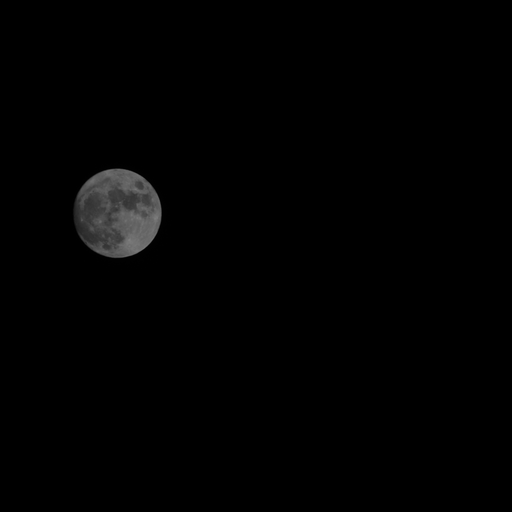
\includegraphics[scale=0.2]{img/best-boss-5162} & 
		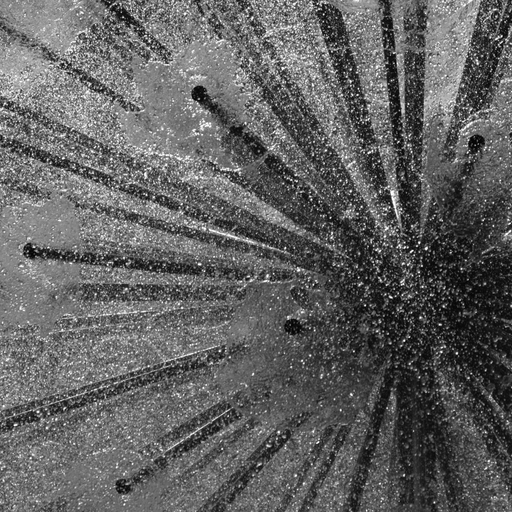
\includegraphics[scale=0.2]{img/worst-boss-1377} \\
		
		
		BOWS2 & 1478.tiff& 5547.tiff\\
		 & 
		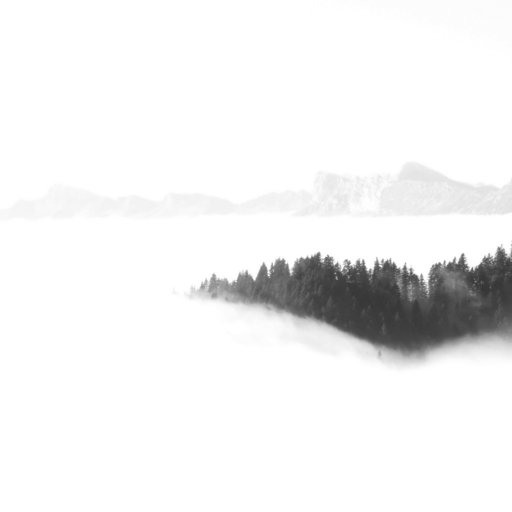
\includegraphics[scale=0.2]{img/best-bows2-1478} & 
		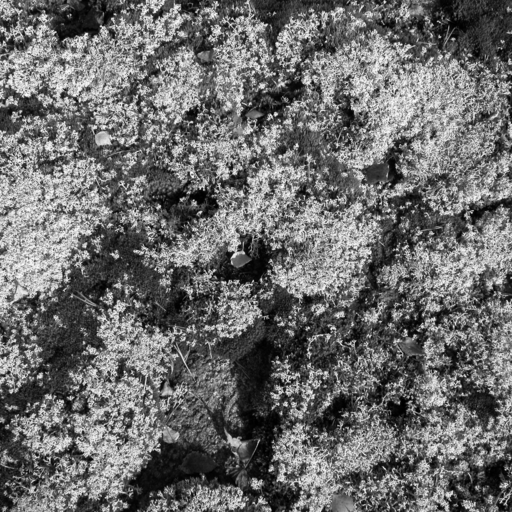
\includegraphics[scale=0.2]{img/worst-bows2-5547} \\
		
		
%		UCID & 00379.tiff& 00341.tiff\\
%		 & 
%		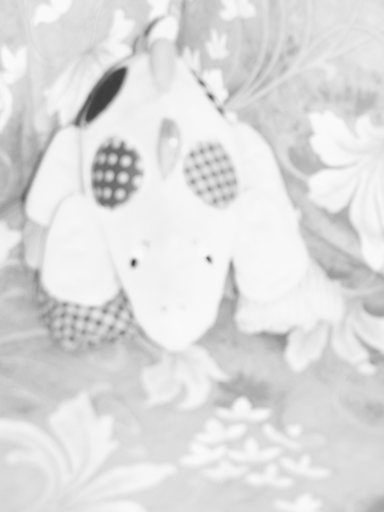
\includegraphics[scale=0.2]{img/best-ucid-00379} & 
%		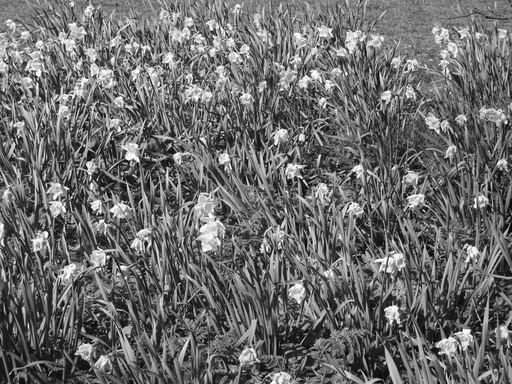
\includegraphics[scale=0.2]{img/worst-ucid-00341} \\
		
		
		USC-SIPI & 7.1.02.tiff& 1.2.05.tiff\\
		 &
		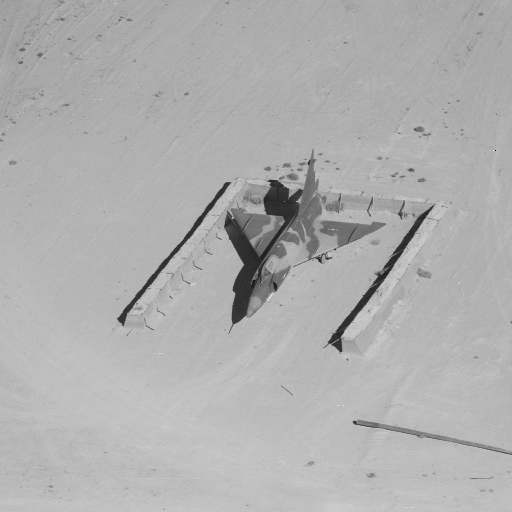
\includegraphics[scale=0.2]{img/best-usc-7.1.02} & 
		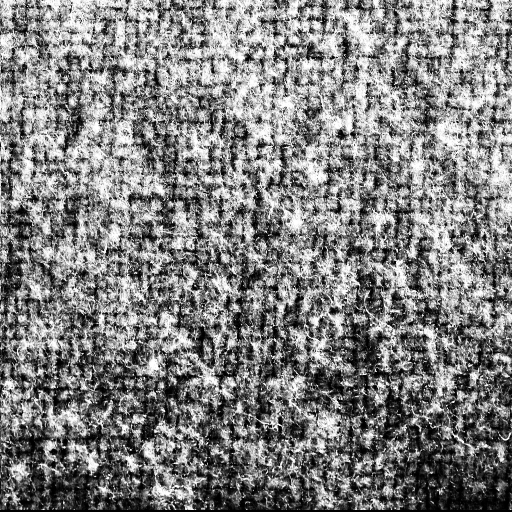
\includegraphics[scale=0.2]{img/worst-usc-1.2.05} \\
		\bottomrule
	\end{tabular}
	\caption{Best and worst cases.}
	\label{fig:bestworst}
\end{figure}

%\begin{figure}
%	
%	\begin{subfigure}{.25\textwidth}
%		\scriptsize
%		
\includegraphics[width=\textwidth]{img/best-usc-gray21.512}
%		\caption{best - gray21.512.tiff}
%	\end{subfigure}
%	\begin{subfigure}{.25\textwidth}
%		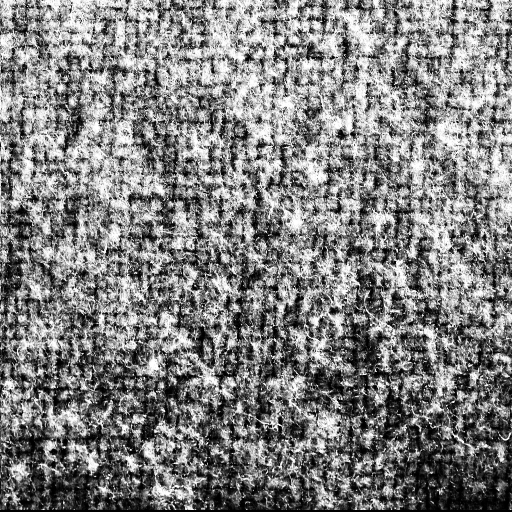
\includegraphics[width=\textwidth]{img/worst-usc-1.2.05}
%		\caption{worst - 1.2.05.tiff}
%	\end{subfigure}
%	\begin{subfigure}{.25\textwidth}
%		
\includegraphics[width=\textwidth]{img/best-usc-gray21.512}
%		\caption{best - gray21.512.tiff}
%	\end{subfigure}
%	\begin{subfigure}{.25\textwidth}
%		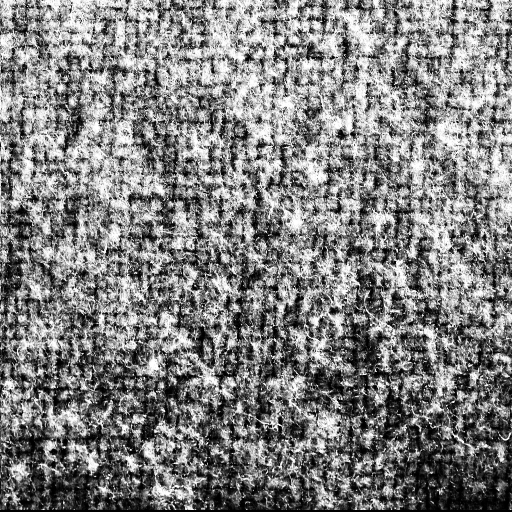
\includegraphics[width=\textwidth]{img/worst-usc-1.2.05}
%		\caption{worst - 1.2.05.tiff}
%	\end{subfigure}
%%	\subcaption{subcaption here}
%%	\subcaption*{heading}
%	\caption{USC-SIPI}
%\end{figure}

\CatchFileDef{\singlemanmsb}{single-res-table-msb-Man.tex}{}
\CatchFileDef{\singlemanshr}{single-res-table-shr-Man.tex}{}
\begin{table}
%	\scriptsize
	\centering
	\caption{The encoding result of Man $1024 \times 1024$.}
	\label{tab:man}
	\subcaption{when applying~\cite{Yin2020}.}
	\label{tab:mana}
	\begin{tabular}{crlcccr}
		\toprule 
		$v$ &   \multicolumn{1}{c}{$f_v$} &     \multicolumn{1}{c}{$encode(v)$}  &  $cap(v)$ &    $\vert encode(v) \vert$    & $payload(v)$  & $\Delta$ \\
		\midrule 
		\singlemanmsb
		\bottomrule
		\multicolumn{7}{l}{Average code length per value: $3121506 \divisionsymbol 1046529 = 2.982722$}
	\end{tabular}

	\subcaption{when applying our method.}
	\label{tab:manb}
	\begin{tabular}{crlcccr}
		\toprule 
		$v$ &   \multicolumn{1}{c}{$f_v$} &     \multicolumn{1}{c}{$encode(v)$}  &  $cap(v)$ &    $\vert encode(v) \vert$    & $payload(v)$  & $\Delta$ \\
		\midrule 
		\singlemanshr
		\bottomrule
		\multicolumn{7}{l}{Average code length per value: $3127243 \divisionsymbol 1048506 = 2.982570$}
	\end{tabular}
	
\end{table}





BOSSBase~\cite{Bas2011}
BOWS-2~\cite{bows2007}

%UCID~\cite{Schaefer2003}

The USC-SIPI Image Database~\cite{USC1966}



%\begin{table}
%	\centering
%	\caption{Embedding capacity in bits}
%	\begin{tabular}{ccccc cccc}
%		\toprule
%		           & \multicolumn{4}{c}{Yin et~al.} 
%		           & \multicolumn{4}{c}{Ours}                                                      \\
%		\cmidrule(lr){2-5} \cmidrule(lr){6-9}
%		Test Image & EC                              & LM                       & Extra & bpp   & EC      & LM       & Extra & bpp   \\ 
%		\midrule
%		Lena       & 1470568                         & 793304                   & 52    & 2.583 & 1476577 & 787307   & 73    & 2.628 \\ 
%		Baboon     & 1074384                         & 794941                   & 52    & 1.066 & 1077990 & 789553   & 73    & 1.099 \\
%		Jetplane   & 1587880                         & 793441                   & 52    & 3.030 & 1594681 & 781177   & 73    & 3.102 \\
%		Airplane   & 1659203                         & 682803                   & 52    & 3.724 & 1665774 & 659619 & 73 & 3.837        \\
%		Tiffany    & 1526934                         & 786527                   & 52    & 2.824 & 1533558 & 772751   & 73    & 2.901 \\
%		Man        & 5584907                         & 
%		\makecell{3121508\\(3121506)}&
%		\makecell{52\\(54)}&
%		2.349&5595967&3127374&75&2.354\\
%		\bottomrule
%	\end{tabular}
%\end{table}







%\begin{table}
%	\scriptsize
%	\centering
%	\caption{Embedding capacity in bits (Ours/Yin et~al./$\Delta$)}
%	\begin{tabular}{cccccc}
%		\toprule
%		Image & Capacity                     & Encoded Label Map               & Header  & Reference& BPP.      \\ 
%		\midrule
%		Airplane  & 1665576/1659203/+6373	& 659628/682803/-23175	& 53/52/+1	& 192/8184/-7992	& 3.837/3.725/+0.113	 	\\
%		Baboon    & 1077790/1074384/+3406	& 789559/794941/-5382	& 53/52/+1	& 192/8184/-7992	& 1.100/1.066/+0.034	 	\\
%		Jetplane  & 1594482/1587880/+6602	& 781183/793441/-12258	& 53/52/+1	& 192/8184/-7992	& 3.102/3.031/+0.072	 	\\
%		Lena      & 1476381/1470568/+5813	& 787311/793304/-5993	& 53/52/+1	& 192/8184/-7992	& 2.629/2.584/+0.045	 	\\
%		Man       & 5595769/5584907/+10862	& 3127379/3121506/+5873	& 53/54/-1	& 192/16376/-16184	& 2.354/2.349/+0.005	 	\\
%		Tiffany   & 1533366/1526934/+6432	& 772757/786527/-13770	& 53/52/+1	& 192/8184/-7992	& 2.901/2.824/+0.077	 	\\
%		 
%%		\midrule
%%		Man        & 5595967/5584907/+11060 & 
%%			\makecell{3127374/3121508/+5866\\(3127374/3121506/+5868)} &
%%			\makecell{75/52/23\\(75/54/21)} & 
%%			2.354/2.349/+0.005\\
%		\bottomrule
%	\end{tabular}
%\end{table}

%\begin{table}
%	\scriptsize
%	\centering
%	\caption{Huffman Coding of Lena $512 \times 512$}
%	
%	
%	
%	\subcaption{Ours}
%	\begin{tabular}{crlccrr}
%		\toprule 
%		$t$ &   \multicolumn{1}{c}{$f_t$} &     \multicolumn{1}{c}{Code}   &  Cap.&    Len.    & Payload  & $\Delta$ \\ 
%		%------------------------------------------------------
%		\midrule 
%%		0 &     9818 & 11110    &        1 &        5 &       -4 &   -39272  \\ 
%%		1 &     9742 & 11111    &        2 &        5 &       -3 &   -29226  \\ 
%%		2 &    15247 & 1110     &        3 &        4 &       -1 &   -15247  \\ 
%%		3 &    33246 & 101      &        4 &        3 &        1 &    33246  \\ 
%%		4 &    44509 & 01       &        5 &        2 &        3 &   133527  \\ 
%%		5 &    53359 & 00       &        6 &        2 &        4 &   213436  \\ 
%%		6 &    41758 & 100      &        7 &        3 &        4 &   167032  \\ 
%%		7 &    24353 & 1101     &        8 &        4 &        4 &    97412  \\ 
%%		8 &    29089 & 1100     &        8 &        4 &        4 &   116356  \\ 
%%		\midrule 
%%		Total &   261121 & & &  1470568 &   793304 &   677264 \\ 
%
%\singlelenashr
%
%		\bottomrule   
%	\end{tabular}
%	
%	
%	\subcaption{Yin et al}
%	\begin{tabular}{crlccrr}
%		\toprule 
%		$t$ &   \multicolumn{1}{c}{$f_t$} &     \multicolumn{1}{c}{Code}  &  Cap. &    Len.    & Payload  & $\Delta$ \\
%		%------------------------------------------------------
%		\midrule 
%%		0 &     9867 & 10111    &        1 &        5 &       -4 &   -39468 \\ 
%%		1 &     9751 & 10110    &        2 &        5 &       -3 &   -29253 \\ 
%%		2 &    15321 & 1010     &        3 &        4 &       -1 &   -15321 \\ 
%%		3 &    33303 & 100      &        4 &        3 &        1 &    33303 \\ 
%%		4 &    44679 & 111      &        5 &        3 &        2 &    89358 \\ 
%%		5 &    53604 & 00       &        6 &        2 &        4 &   214416 \\ 
%%		6 &    41938 & 110      &        7 &        3 &        4 &   167752 \\ 
%%		7 &    24452 & 010      &        8 &        3 &        5 &   122260 \\ 
%%		8 &    29203 & 011      &        8 &        3 &        5 &   146015 \\ 
%%		\midrule 
%%		Total &   262118 & & &  1476369 &   787307 &   689062 \\ 
%
%
%\singlelenamsb
%
%	\bottomrule
%	&&&&&&\\
%
%%		\midrule 
%%		$\Delta$ &   +997 & & &  +5801 &   -5997 &   +11798 \\ 
%\singlelenadif
%		\bottomrule 
%	\end{tabular}
%\end{table}